\documentclass[11pt,a4paper]{article}
\usepackage[margin=23mm]{geometry}
\usepackage[T1]{fontenc}
\usepackage[utf8]{inputenc}
\usepackage{lmodern,microtype}
\usepackage{amsmath,amssymb}
\usepackage{booktabs,tabularx,array}
\usepackage{graphicx,tikz}
\usetikzlibrary{arrows.meta,positioning}
\usepackage[font=small,labelfont=bf]{caption}
\usepackage{xcolor,listings,xurl}
\usepackage{hyperref}
\hypersetup{colorlinks=true,linkcolor=blue!40!black,citecolor=blue!40!black,
  urlcolor=blue!40!black,pdftitle={Team possession from automatic football tracking},
  pdfauthor={Barca4Ever}}
\lstset{basicstyle=\ttfamily\footnotesize,columns=fullflexible,keepspaces=true,
  frame=single,framerule=0.2pt,rulecolor=\color{black!25},breaklines=true,
  aboveskip=7pt,belowskip=7pt}
\setlength{\parskip}{3pt}
\setlength{\parindent}{0pt}
\setlength{\textfloatsep}{12pt}
\setlength{\intextsep}{10pt}
\setlength{\tabcolsep}{5pt}

\title{\vspace{-1.2cm}Team possession from automatic football tracking\\
  \large V5 technical report}
\author{Barca4Ever}
\date{More Than A Hack 2027 -- Initial Challenge\\11 November 2026}

\begin{document}
\maketitle
\vspace{-0.7cm}
\begin{abstract}
We estimate team possession from player and ball tracks with missing observations
and fragmented player identities. V5 combines a geometry classifier with a
trajectory network, then uses learned directed transitions to decode possession
spells. The final model was fitted on four licensed external matches and selected
using a fifth. In reciprocal cross-validation within the four fitting matches,
spellF1 was 0.7133 on clean tracking and 0.5344 with simulated noise. The collection
has been inspected repeatedly during development, so these are development
results with limited independent evidence. Noisy short possessions remain the
main weakness. Our pipeline runs offline on a CPU and produces one
label for each of the 199,319 tactical-video frames.
\end{abstract}

\section{Task and evaluation}
The output is a sequence of home possession ($H$), away possession ($A$), dead ball
($D$), and abstention ($X$). A useful estimate must recover when possessions start
and end. Frame accuracy can hide errors on brief possessions, while rapidly
alternating labels can create possessions that never occurred.

The organizer ranks submissions by \texttt{spellF1}, with frame-level
\texttt{macroF1} breaking ties. A possession spell is a
maximal uninterrupted $H$ or $A$ interval inside a scored reference span. Predicted
and reference spells are matched one-to-one within the same team by temporal
intersection-over-union (IoU). F1 is computed at IoU thresholds
$0.3,0.4,0.5,0.6,0.7$ and averaged. Dead-ball intervals are excluded from the spell
list. Unknown reference spans are excluded. Predicted $X$ values are forward-filled,
with leading abstentions back-filled inside each valid span. The separate short-recovery count
uses spells shorter than two seconds and IoU $0.5$. These counts are distinct from
the multi-threshold headline score.

V5 takes tactical player and ball XY positions and team assignments. We chose to
work from these tracks. Video, Smart Tagging, broadcast tracking and homography
are outside this implementation. All fitting, selection and quality evaluation
use external labels. The supplied match is used for local inference.

\section{Method}
Figure~\ref{fig:pipeline} shows the inference path. Geometry supplies direct spatial
evidence. The trajectory network adds local motion and observation history. The
transition model helps the decoder place changes without accepting every brief
fluctuation in the frame probabilities.

\begin{figure}[ht]
\centering
\resizebox{0.98\linewidth}{!}{%
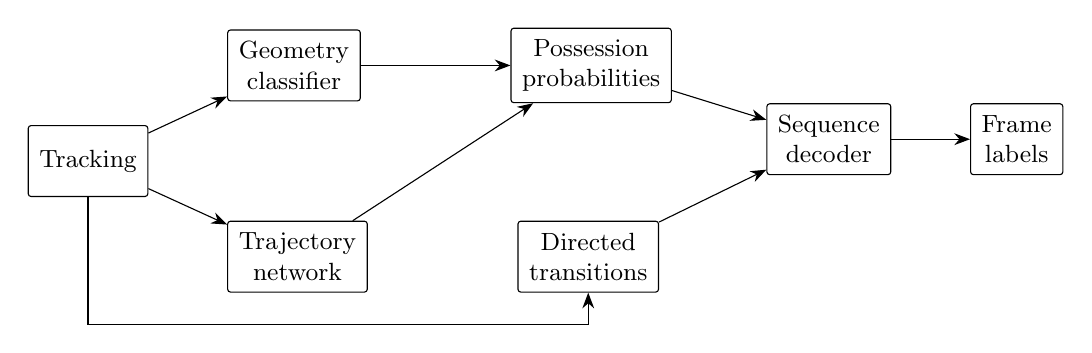
\begin{tikzpicture}[node distance=3mm and 10mm,
  box/.style={draw,rounded corners=1pt,align=center,font=\small,
    minimum height=9mm,inner sep=4pt},
  arr/.style={-{Stealth[length=2mm]},thin}]
  \node[box] (input) {Tracking};
  \node[box,above right=of input] (geo) {Geometry\\classifier};
  \node[box,below right=of input] (net) {Trajectory\\network};
  \node[box,right=19mm of geo] (prob) {Possession\\probabilities};
  \node[box,right=19mm of net] (edge) {Directed\\transitions};
  \node[box,below right=0mm and 12mm of prob] (decode) {Sequence\\decoder};
  \node[box,right=of decode] (out) {Frame\\labels};
  \draw[arr] (input) -- (geo);
  \draw[arr] (input) -- (net);
  \draw[arr] (geo) -- (prob);
  \draw[arr] (net) -- (prob);
  \draw[arr] (input.south) |- ([yshift=-4mm]net.south) -| (edge.south);
  \draw[arr] (prob) -- (decode);
  \draw[arr] (edge) -- (decode);
  \draw[arr] (decode) -- (out);
\end{tikzpicture}}
\caption{V5 inference. The trajectory branch is inspired by contact modeling but
is trained on possession and ball-status labels, without touch-level supervision.}
\label{fig:pipeline}
\end{figure}

\subsection{Input representation}
The source tracks are sampled at 25 Hz. The loader maps source record 1 to output frame 0, converts normalized positions
to pitch-centred metres, and checks record order and slot counts. Slots are
track fragments rather than stable player identities. The network retains all
observed actors in padded team groups and masks missing actors. Goalkeeper-role
inputs stay zero.

Ball gaps of up to two seconds are linearly interpolated between observed
endpoints. Longer gaps remain missing. Raw visibility and time since/until a ball
observation accompany the filled coordinates, so interpolation does not erase
the original missingness. A complete player-tracking outage of at least ten
seconds receives $X$ and separates inference blocks. Missing ball observations
alone do not assign $D$.

\subsection{Possession probabilities}
The geometry branch is a histogram gradient boosting classifier over 59 spatial,
motion and visibility features. The neural branch adapts the shared trajectory
temporal convolutional network (TCN) and ball-query attention approach of Borghesi et al.~\cite{borghesi}. We
implemented and trained this branch ourselves. The authors' original weights and
confidential training data were unavailable.

The network predicts dead probability $d_t$ and conditional home probability
$h_t$. Its joint probabilities are
\begin{equation}
q_t=\big((1-d_t)h_t,\;(1-d_t)(1-h_t),\;d_t\big),\qquad
p_t=\tfrac12 g_t+\tfrac12 q_t,
\end{equation}
where $g_t$ is the geometry classifier output in $H,A,D$ order. The home loss is
masked on dead-ball labels.

The TCN uses width 64 and six causal blocks with kernel size 2 and dilations
$1,2,4,8,16,32$. A target-frame multilayer perceptron (MLP) and distance-biased attention add local
geometry. There are 20 input channels, including raw visibility and observation
gap timing. Inputs are sampled at 16 Hz using actual elapsed source time for
velocity. A window contains 64 samples with zero-based target index 47. It therefore
includes about one second of future trajectories. Gap features can use up to ten
seconds of future observation evidence. This is an offline method.

\subsection{Changes of possession}
A second boosting model estimates the six ordered changes between $H,A,D$, plus
background. It uses 293 geometry/context features, with before, after and signed
differences at offsets $\pm2,6,12$ source frames. Training gives transition
examples extra weight, so its scores are uncalibrated evidence.

\begin{samepage}
For a sequence of $T$ frames, the decoder selects
\begin{equation}
\hat y=\operatorname*{arg\,max}_{y\in\{H,A,D\}^T}
\left[\sum_{t=1}^{T}\log p_t(y_t)-
\sum_{t=2}^{T}\mathbf{1}[y_t\ne y_{t-1}]
\frac{16}{1+8b_t(y_{t-1},y_t)}\right],
\end{equation}
where $b_t(i,j)$ is the directed transition score. A plausible $H$-to-$A$ change
reduces that switch cost specifically. The decoder is run separately in each
tracking block.
\end{samepage}

\section{Experiments and results}
\subsection{External data and selection}
We use IDSSE, the public DFL/Sportec dataset described by Bassek et
al.~\cite{bassek,idsse}. The reference labels are the provider's
\texttt{BallPossession} and \texttt{BallStatus} fields. Inactive ball status maps
to $D$, live possession 1/2 to $H/A$, and unknown to $X$. Labels are isolated from
features. The data are licensed under CC BY 4.0. Our changes include parsing,
feature construction, simulated corruption and model training.

\begin{table}[ht]
\centering\small
\begin{tabularx}{\linewidth}{@{}lX@{}}
\toprule
Role & Matches \\
\midrule
Final fitting & J03WOH, J03WOY, J03WPY, J03WQQ \\
Selection & J03WR9 \\
Reused regression & J03WMX, J03WN1 \\
\bottomrule
\end{tabularx}
\caption{Roles of the seven external matches. Both halves stay with their match.}
\label{tab:split}
\end{table}

The deployed model uses the four fitting matches. Cross-validation within those
four fits WOH/WOY and evaluates WPY/WQQ, then reverses. Each fold excludes its
evaluated matches from every learned component, including the neural initializer.
The two regression matches were originally held out, then reused during
development. All seven matches have now been inspected repeatedly. Fitting
exclusion within a fold does not make this collection an independent final test.

We selected input rate and mixture weights on WR9. The composite had the highest
WR9 spellF1 among candidates that passed their predeclared clean/noisy
cross-validation and regression acceptance checks. The
\href{https://github.com/aqaPayam/Barca4Ever/blob/main/MULTIAGENT_SELECTION_PROTOCOL.md}{selection protocol}
records those comparisons and tie-breaking rules. Its neural branch was fine-tuned for two
epochs of 100,000 fresh references, sampled 75\% by eligible frames and 25\% by
team spells. Detailed configurations, training seeds, checkpoint lineage and
rejected alternatives are recorded in \texttt{V5\_MODEL\_GUIDE.md} and the
\texttt{MULTIAGENT\_RESULTS.md}.

\subsection{Matched comparisons}
V4.1 is the preceding geometry/trajectory pipeline with destination-based boundary
scores. V5 adds raw observation-confidence channels, elapsed-time velocity
correction, fresh training references and directed transitions. The table compares
complete pipelines rather than isolating each change.

We use the same labels and corruption settings for each paired comparison.
Synthetic noise adds 0.25 m player jitter, 0.35 m ball jitter, 5\% player dropout
and contiguous ball gaps of 15--84 source frames. Scores below average halves
equally, while short-spell hits are pooled.

\begin{table}[ht]
\centering
\begin{tabular}{@{}llrrrr@{}}
\toprule
 & & \multicolumn{2}{c}{spellF1} & \multicolumn{2}{c}{Short hits / total} \\
\cmidrule(lr){3-4}\cmidrule(l){5-6}
Comparison & View & V4.1 & V5 & V4.1 & V5 \\
\midrule
Cross-validation & Clean & 0.7105 & 0.7133 & 191/463 & 206/463 \\
Cross-validation & Noisy & 0.5329 & 0.5344 & 79/463 & 80/463 \\
Reused regression & Clean & 0.6808 & 0.6847 & 128/362 & 132/362 \\
Reused regression & Noisy & 0.4968 & 0.5140 & 64/362 & 71/362 \\
\bottomrule
\end{tabular}
\caption{External development results. Short hits use duration below two seconds
and IoU 0.5; spellF1 averages the five thresholds defined in Section 1.}
\label{tab:results}
\end{table}

\begin{samepage}
The noisy cross-validation gain is 0.0015, with one additional short possession
recovered. Noisy reused regression shows a larger difference. Repeated use of all
seven matches limits the independent evidence these comparisons provide.
\end{samepage}

\section{Limitations and reproduction}
V5 recovered 80 of 463 short possessions in noisy cross-validation. Brief
turnovers remain difficult, especially when ball observations are missing or
actor trajectories are fragmented. The corruption model does not cover every
real tracking failure. XY positions also leave whistles, aerial contact and body
orientation ambiguous. Exact nearest-player ties retain the trained slot-order
convention. Finally, one provider and seven repeatedly inspected matches give
limited evidence about transfer to the competition match.

The repository includes the trained artifact and pinned Python 3.12 CPU
dependencies. From its root, a POSIX shell can regenerate the file with
\begin{lstlisting}
python -m pip install -r requirements-contact.txt
python refined_infer.py \
  --model models/external_v5.joblib \
  --data-dir /local/bundle \
  --out local_outputs/Barca4Ever.csv
python evaluation/validate_submission.py local_outputs/Barca4Ever.csv
\end{lstlisting}
The bundle contains \texttt{tactical/BAR-ATH\_tactical\_atd.xml} and its
\texttt{.txt} tracking file. Windows users can run
\texttt{Run-Barca4Ever.ps1}. CPU inference uses four threads. The output manifest
records model and CSV hashes.

The November 11 release passed 85 synthetic tests and a 199,319-frame generated
match through the launcher, V5 inference and the organizer's format validator.
Earlier evidence records four external CPU parity comparisons and the original
82-test suite. These are software checks. The possession-quality evidence is
Table~\ref{tab:results}. The competition score awaits the organizer's private
evaluation.

Challenge inputs, predictions and local logs are excluded from the public
package. Inference performs no fitting or calibration, and predictions were not
checked against the supplied video or ground truth. The organizers prohibit
uploading their match data or extracts to hosted AI services. Dataset attribution
must accompany the trained artifacts.

\smallskip
\noindent\textbf{Repository}\quad
\url{https://github.com/aqaPayam/Barca4Ever}

\begin{thebibliography}{9}
\small
\bibitem{borghesi}
M. Borghesi, L. D. Costa, L. Morra and F. Lamberti.
Using Temporal Convolutional Networks to estimate ball possession in soccer
games. \emph{Expert Systems with Applications}, 223, 119780, 2023.
\href{https://doi.org/10.1016/j.eswa.2023.119780}{doi:10.1016/j.eswa.2023.119780}.

\bibitem{bassek}
M. Bassek, R. Rein, H. Weber and D. Memmert.
An integrated dataset of spatiotemporal and event data in elite soccer.
\emph{Scientific Data}, 12, 195, 2025.
\href{https://doi.org/10.1038/s41597-025-04505-y}{doi:10.1038/s41597-025-04505-y}.

\bibitem{idsse}
IDSSE dataset. Original data from DFL / Sportec Solutions.
\href{https://doi.org/10.6084/m9.figshare.28196177}{doi:10.6084/m9.figshare.28196177}.
Licensed under \href{https://creativecommons.org/licenses/by/4.0/}{CC BY 4.0}.
\end{thebibliography}
\end{document}
